% UBT-AI-PROVENANCE-BEGIN
% schema: ubt-ai-provenance/v1
% tier: C_working
% ai_assistance: disclosed
% human_review: risk-based
% editorial_responsibility: Ing. David Jaroš
% policy: ../../../AI_PROVENANCE.md
% notice: Working material; exhaustive human review is not claimed.
% UBT-AI-PROVENANCE-END

\section*{Jak tento text číst}
\addcontentsline{toc}{section}{Jak tento text číst}
Tento text nevychází z předpokladu, že si čtenář pamatuje diferenciální geometrii.
Je určen člověku, který dobře chápe strukturu problému, ale ztrácí se v množství
indexů a v podobně vypadajících antisymetrických objektech. Cílem není naučit se
vzorce nazpaměť. Cílem je získat několik obrazů, ze kterých lze vzorce znovu
odvodit.

\begin{memorybox}{Čtyři věty, které mají zůstat v hlavě}
\begin{enumerate}[leftmargin=*,itemsep=0.25em]
  \item Christoffelovy symboly jsou pro každý směr pohybu jedna matice míchající složky vektoru.
  \item Torze měří nedovření dvou po sobě provedených infinitesimálních kroků.
  \item Operátor $\operatorname{rot}$ měří lokální cirkulaci vektorového pole; není to torze.
  \item Antikomutátor v UBT vybírá symetrický metrický kanál; jeho antisymetrický doplněk není torze.
\end{enumerate}
\end{memorybox}

\section{Nejdříve indexy: proč jich je tolik}

\subsection{Index není mocnina}
V zápisu $V^\mu$ není $\mu$ exponent. Je to štítek složky. Ve čtyřrozměrném
časoprostoru může $\mu$ nabývat hodnot $0,1,2,3$:
\[
  V^\mu=(V^0,V^1,V^2,V^3).
\]
Horní a dolní index označují dva různé typy transformačního chování. Pro první
čtení stačí vědět, že metrika umí index snížit nebo zvýšit:
\[
  V_\mu=g_{\mu\nu}V^\nu,
  \qquad
  V^\mu=g^{\mu\nu}V_\nu.
\]
To není kosmetika, ale pro intuitivní orientaci lze horní index číst jako
``výstupní složku'' a dolní jako ``vstupní slot''.

\subsection{Volný a sčítaný index}
V rovnici
\[
  W^\rho=M^\rho{}_{\nu}V^\nu
\]
je $\rho$ volný index: na obou stranách říká, kterou složku výsledku počítáme.
Index $\nu$ se opakuje, a proto se přes něj sčítá:
\[
  W^\rho=\sum_{\nu=0}^{3}M^\rho{}_{\nu}V^\nu.
\]
Je to obyčejné násobení matice vektorem, pouze zapsané úsporněji.

\begin{memorybox}{Pravidlo pro čtení indexů}
Index, který se v jednom členu objeví dvakrát, je obvykle sčítaný. Index, který
zůstane jednou, označuje složku výsledku. Nejprve proto nečti symboly, ale
zakroužkuj opakované indexy.
\end{memorybox}

\subsection{Co znamenají tři indexy Christoffelova symbolu}
Definiční vztah je
\[
  \nabla_{\partial_\mu}\partial_\nu
  =\Gamma^\rho{}_{\mu\nu}\,\partial_\rho.
\]
Tuto rovnici lze přečíst slovně:
\begin{quote}
Když se pohybuji ve směru $\mu$ a sleduji bázový vektor $\partial_\nu$, jeho
změna má složku ve výstupním směru $\rho$ velikosti
$\Gamma^\rho{}_{\mu\nu}$.
\end{quote}
Role indexů tedy jsou:
\[
\boxed{
\begin{array}{ccl}
\mu &:& \text{směr, ve kterém derivujeme},\\
\nu &:& \text{vstupní složka nebo bázový vektor},\\
\rho&:& \text{výstupní složka po promíchání}.
\end{array}}
\]

Pro pevné $\mu$ definujme matici
\[
  (\Gamma_\mu)^\rho{}_{\nu}:=\Gamma^\rho{}_{\mu\nu}.
\]
Ve čtyřech rozměrech tedy můžeme $\Gamma$ chápat jako čtveřici matic
\[
  \Gamma_0,\ \Gamma_1,\ \Gamma_2,\ \Gamma_3,
  \qquad \Gamma_\mu\in\operatorname{Mat}(4,\mathbb R).
\]
Kovariantní derivace vektoru pak opravdu vypadá jako maticová rovnice:
\[
  \nabla_\mu V=\partial_\mu V+\Gamma_\mu V,
\]
nebo po složkách
\[
  \nabla_\mu V^\rho
  =\partial_\mu V^\rho+\Gamma^\rho{}_{\mu\nu}V^\nu.
\]

\begin{examplebox}{Jak číst jediný prvek}
Symbol $\Gamma^2{}_{01}$ znamená: při pohybu ve směru $x^0$ se vstupní bázový
vektor $\partial_1$ mění také do směru $\partial_2$. Není to třetí derivace ani
prvek nějaké tajemné trojrozměrné matice. Je to prvek řádku $2$, sloupce $1$ v
matici $\Gamma_0$.
\end{examplebox}

\subsection{Proč Christoffelovy symboly nejsou samy křivost}
V polárních souřadnicích jsou některé Christoffelovy symboly nenulové už v
obyčejné ploché rovině. Důvodem je, že se směry ``radiálně'' a ``po kružnici''
mění z bodu do bodu. Spojení tedy popisuje změnu báze. Křivost je až výsledek
transportu kolem uzavřené smyčky.

Christoffelovy symboly navíc samy nejsou tenzor: při změně souřadnic dostávají
nehomogenní korekční člen. Tenzorové jsou až z nich složené objekty, například
torze a křivost.

\section{Tři druhy antisymetrie, které se nesmějí zaměnit}

Mnoho zmatku vzniká proto, že torze, rotace a komutátor používají rozdíl dvou
výrazů s prohozenými indexy. Podobný zápis však neznamená stejný objekt.

\subsection{Operátor rot: víření vektorového pole}
V trojrozměrném eukleidovském prostoru je
\[
  \operatorname{rot}\mathbf A=\nabla\times\mathbf A.
\]
Po složkách:
\[
  (\operatorname{rot}\mathbf A)^i
  =\varepsilon^{ijk}\partial_j A_k.
\]
Například jeho třetí složka je
\[
  (\operatorname{rot}\mathbf A)^3
  =\partial_1A_2-\partial_2A_1.
\]
Rot tedy porovnává, jak se složky jednoho vektorového pole mění ve dvou
prostorových směrech. Měří lokální cirkulaci: zda má malé lopatkové kolečko
vložené do pole tendenci se otáčet.

Ve čtyřrozměrném zápisu je přirozenější antisymetrický tenzor
\[
  F_{\mu\nu}=\partial_\mu A_\nu-\partial_\nu A_\mu.
\]
Obvyklý trojrozměrný rot je prostorová duální reprezentace části $F_{ij}$.
Proto elektromagnetický tenzor pole obsahuje elektrické i magnetické složky,
zatímco školní rot je pouze trojrozměrný obraz.

\begin{examplebox}{Pole s konstantním rotem}
Pro
\[
  \mathbf A(x,y,z)=\left(-\frac y2,\frac x2,0\right)
\]
platí
\[
  \operatorname{rot}\mathbf A=(0,0,1).
\]
Pole obíhá kolem osy $z$. To ale nic neříká o torzi časoprostorového spojení.
Jsme stále v obyčejném plochém prostoru a pouze jsme zvolili vířivé pole.
\end{examplebox}

\subsection{Torze: nedovření infinitesimálních kroků}
Torze spojení je definována bez souřadnic jako
\[
  T(X,Y)=\nabla_XY-\nabla_YX-[X,Y].
\]
V souřadnicové bázi $[\partial_\mu,\partial_\nu]=0$, a proto
\[
  \boxed{
  T^\rho{}_{\mu\nu}
  =\Gamma^\rho{}_{\mu\nu}-\Gamma^\rho{}_{\nu\mu}.}
\]
Torze je antisymetrická v indexech $\mu,\nu$, ale tyto indexy nyní označují
pořadí dvou geometrických posunů. Nenulová torze znamená, že cesta ``nejprve
$\mu$, potom $\nu$'' se infinitesimálně nesejde s cestou ``nejprve $\nu$,
potom $\mu$''.

\begin{center}
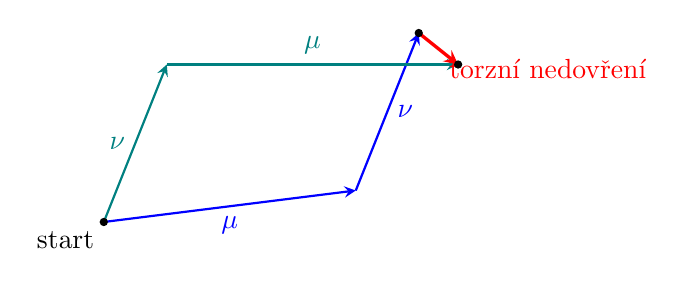
\begin{tikzpicture}[scale=1.0,>=stealth]
  \coordinate (O) at (0,0);
  \coordinate (A) at (3.2,0.4);
  \coordinate (B) at (0.8,2.0);
  \coordinate (C) at (4.0,2.4);
  \coordinate (Cp) at (4.5,2.0);
  \draw[->,thick,blue] (O)--(A) node[midway,below] {$\mu$};
  \draw[->,thick,blue] (A)--(C) node[midway,right] {$\nu$};
  \draw[->,thick,teal] (O)--(B) node[midway,left] {$\nu$};
  \draw[->,thick,teal] (B)--(Cp) node[midway,above] {$\mu$};
  \draw[->,very thick,red] (C)--(Cp) node[midway,below right] {torzní nedovření};
  \fill (O) circle (1.5pt) node[below left] {start};
  \fill (C) circle (1.5pt);
  \fill (Cp) circle (1.5pt);
\end{tikzpicture}
\end{center}

V tetrádovém jazyce je stejná informace zapsána Cartanovou rovnicí
\[
  \boxed{T^a=de^a+\omega^a{}_b\wedge e^b.}
\]
Zde $e^a$ je lokální rámec a $\omega^a{}_b$ spinové spojení. Pokud $T^a=0$ a
spojení zachovává metriku, dostáváme jednoznačné Levi--Civitovo spojení.

\subsection{Křivost: změna po návratu kolem smyčky}
Křivost měří jiný efekt: vektor po paralelním transportu kolem malé uzavřené
smyčky změní směr. Symbolicky
\[
  [\nabla_\mu,\nabla_\nu]V^\rho
  =R^\rho{}_{\sigma\mu\nu}V^\sigma
   -T^\lambda{}_{\mu\nu}\nabla_\lambda V^\rho.
\]
V beztorzní větvi druhý člen zmizí. Křivost je tedy analogická holonomii kolem
smyčky, torze translačnímu nedovření a rot lokálnímu víření konkrétního pole.

\begin{memorybox}{Jednověté rozlišení}
\begin{itemize}[leftmargin=*,itemsep=0.2em]
  \item $\operatorname{rot}\mathbf A$: víří konkrétní vektorové pole $\mathbf A$.
  \item $T$: dva geometrické posuny se translačně nedovřou.
  \item $R$: vektor se po oběhu smyčky vrátí změněný.
\end{itemize}
\end{memorybox}

\section{Nediagonální složky nejsou torze}
Matice metriky může mít nediagonální složky $g_{\mu\nu}$ pro $\mu\neq\nu$.
Ty vyjadřují, že zvolená souřadnicová osa není ortogonální k jiné ose, případně
že se v zápisu mísí čas a prostor. Samy o sobě nic nedokazují o torzi.

Stejně tak může mít matice $\Gamma_\mu$ mnoho nediagonálních prvků a přitom
může být torze nulová. Torze nezkoumá diagonálu matice. Zkoumá prohození dvou
směrových indexů:
\[
  \Gamma^\rho{}_{\mu\nu}
  \quad\hbox{oproti}\quad
  \Gamma^\rho{}_{\nu\mu}.
\]
Tato oprava intuice je důležitá: ``míchání složek'' je vlastnost spojení,
zatímco torze je specifická antisymetrie pořadí geometrických posunů.

\section{Antikomutátor a komutátor}

Pro dva obecně nekomutující objekty $A,B$ definujeme
\[
  \{A,B\}=AB+BA,
  \qquad
  [A,B]=AB-BA.
\]
Antikomutátor je symetrický při záměně $A\leftrightarrow B$, komutátor je
antisymetrický. Obě operace jsou čistě algebraické: nepotřebují derivaci ani
spojení.

U Pauliho matic například platí
\[
  \{\sigma_i,\sigma_j\}=2\delta_{ij}\mathbf 1,
  \qquad
  [\sigma_i,\sigma_j]=2i\varepsilon_{ijk}\sigma_k.
\]
Symetrická část dává skalární produkt, antisymetrická část orientovanou rotační
strukturu. Stejná logika stojí za tetrádovým čtením metriky v UBT.

\section{UBT: plný součin, metrický kanál a bivektorový kanál}

Definujme covariantní tetrádové směry
\[
  E_\mu=\mathcal N_0^{-1/2}D_\mu\Theta.
\]
Plný uspořádaný biquaternionový součin je
\[
  \mathfrak G_{\mu\nu}=E_\mu^\sharp E_\nu.
\]
Rozloží se jednoznačně na symetrickou a antisymetrickou část:
\[
  \mathfrak G_{\mu\nu}
  =\gamma_{\mu\nu}\mathbf 1+\Sigma_{\mu\nu},
\]
kde
\[
  \boxed{
  \gamma_{\mu\nu}\mathbf 1
  =\frac12\left(E_\mu^\sharp E_\nu+E_\nu^\sharp E_\mu\right)}
\]
a
\[
  \boxed{
  \Sigma_{\mu\nu}
  =\frac12\left(E_\mu^\sharp E_\nu-E_\nu^\sharp E_\mu\right).}
\]
Na Lorentzovsky reálné větvi je $\gamma_{\mu\nu}=g_{\mu\nu}$ běžná metrika.
Antikomutátor tedy není torze: je to algebraický projektor na centrální
symetrický kanál.

\begin{center}
\resizebox{0.94\textwidth}{!}{%
\begin{tikzpicture}[node distance=1.2cm and 1.7cm,>=stealth]
\node[draw,rounded corners,fill=gray!8,minimum width=4.3cm,minimum height=1cm] (full)
{$E_\mu^\sharp E_\nu$ -- plný uspořádaný součin};
\node[draw,rounded corners,fill=blue!8,below left=of full,minimum width=4.2cm,minimum height=1.2cm,align=center] (sym)
{$\gamma_{\mu\nu}\mathbf1$\\symetrický metrický kanál};
\node[draw,rounded corners,fill=orange!12,below right=of full,minimum width=4.2cm,minimum height=1.2cm,align=center] (asym)
{$\Sigma_{\mu\nu}$\\antisymetrický bivektorový kanál};
\draw[->,thick] (full)--(sym) node[midway,left] {$\tfrac12(X+X^{\rm swap})$};
\draw[->,thick] (full)--(asym) node[midway,right] {$\tfrac12(X-X^{\rm swap})$};
\end{tikzpicture}%
}
\end{center}

\subsection{Proč se antisymetrický kanál neobjeví v obyčejném \texorpdfstring{$ds^2$}{ds2}}
Pro komutující diferenciály platí
\[
  dx^\mu dx^\nu=dx^\nu dx^\mu.
\]
Proto
\[
  \Sigma_{\mu\nu}dx^\mu dx^\nu=0,
\]
neboť antisymetrická $\Sigma$ se kontrahuje se symetrickým součinem
diferenciálů. Plný součin $\mathfrak G$ však nezmizel; pouze jeho antisymetrický
kanál není vidět v běžném kvadratickém délkovém elementu.

\section{Je kandidát neviditelnosti způsoben torzí?}

Krátká odpověď zní: \textbf{ne nutně}. Nejostřejší algebraická podmínka
zkoumaná v UBT je
\[
  \boxed{\gamma_{\mu\nu}=0,
  \qquad \Sigma_{\mu\nu}\neq0.}
\]
Symetrický centrální metrický kanál je nulový, zatímco plná biquaternionová
struktura zůstává aktivní. Tato možnost vzniká z algebraických vlastností
součinů $E_\mu^\sharp E_\nu$, nikoli z definice torze.

Torze však může vstoupit nepřímo, protože
\[
  E_\mu=D_\mu\Theta
\]
závisí na spojení. Torsionální neboli kontorzní část spojení může pomoci
realizovat určitou tetrádu, ovlivnit integrabilitu nebo dynamiku konfigurace.
To ale neznamená, že antisymetrický kanál $\Sigma_{\mu\nu}$ je torze nebo že
nulová metrika automaticky vyžaduje nenulovou torzi.

\begin{memorybox}{Přesná formulace}
Algebraická podmínka $\gamma=0$, $\Sigma\neq0$ sama o sobě neurčuje torzi.
O tom, zda konkrétní konfigurace patří do beztorzní nebo torzní větve, rozhoduje
spojení, integrabilita a dynamické rovnice. Torze může měnit realizovatelnost a
dynamiku pole, ale není totožná s mechanismem symetrického algebraického
zrušení. Stabilní on-shell neviditelné řešení zatím není dokázáno v žádné větvi.
\end{memorybox}

\subsection{Proč to ještě není fyzikální neviditelnost}
Podmínka $\gamma=0$ nebo $\det\gamma=0$ je pouze kinematická a algebraická.
Pro skutečnou neviditelnost by bylo třeba navíc dokázat:
\begin{enumerate}[leftmargin=*]
  \item regulární řešení rovnic pohybu;
  \item stabilitu vůči poruchám;
  \item dobře definovanou akci i při degenerované metrice;
  \item nulové nebo vakuové elektromagnetické rozptylování;
  \item nulovou nebo vakuovou gravitační odezvu vně objektu;
  \item regulární přechod mezi vnitřní a vnější oblastí.
\end{enumerate}
Proto je správný termín \emph{kandidát metrické nullity}, nikoli hotový stroj
neviditelnosti.

\section{Velká srovnávací tabulka}

\begin{center}
\small
\renewcommand{\arraystretch}{1.35}
\begin{tabularx}{\textwidth}{>{\bfseries}p{2.5cm}X X X}
\toprule
Objekt & Z čeho vzniká & Co měří & Co to není\\
\midrule
$\operatorname{rot}\mathbf A$ & antisymetrické derivace složek konkrétního pole & lokální cirkulaci pole & torze geometrie\\
$T^\rho{}_{\mu\nu}$ & antisymetrie spojení v pořadí směrů; obecně $\nabla_XY-\nabla_YX-[X,Y]$ & translační nedovření infinitesimálních kroků & nediagonální část metriky\\
$R^\rho{}_{\sigma\mu\nu}$ & komutátor kovariantních derivací & změnu vektoru po transportu kolem smyčky & algebraický komutátor tetrád\\
$\gamma_{\mu\nu}$ & antikomutátor $E_\mu^\sharp E_\nu$ & symetrický centrální metrický kanál & torze nebo rot\\
$\Sigma_{\mu\nu}$ & komutátorová část $E_\mu^\sharp E_\nu$ & orientovaný algebraický bivektorový kanál & automaticky křivost či torze\\
\bottomrule
\end{tabularx}
\end{center}

\section{Jak spolu objekty přesto souvisejí}
Je užitečné nespadnout ani do opačného extrému: objekty nejsou totožné, ale v
plné teorii spolu komunikují.

\begin{enumerate}[leftmargin=*]
  \item Pole $\Theta$ a spojení určují $E_\mu=D_\mu\Theta$.
  \item Antikomutátor $E_\mu,E_\nu$ určí metrický kanál $\gamma_{\mu\nu}$.
  \item Z metriky a zvolené torze se rekonstruuje metricky kompatibilní spojení.
  \item Komutátor kovariantních derivací určuje křivost tohoto spojení.
  \item Dynamická akce musí rozhodnout, zda je torze nulová, pomocná, nebo
        propagující a zda je metrická nullita fyzikálně přípustná.
\end{enumerate}

Vzniká tedy zpětnovazební smyčka, nikoli identita pojmů:
\[
  \Theta\ \longrightarrow\ E_\mu
  \ \longrightarrow\ (\gamma,\Sigma)
  \ \longleftrightarrow\ (g,\omega,T,R).
\]

\section{Pět malých testů porozumění}

\begin{enumerate}[leftmargin=*]
\item Co znamená $\Gamma^3{}_{21}$?\\
\emph{Odpověď:} V matici $\Gamma_2$ jde o řádek $3$, sloupec $1$. Při derivaci
ve směru $2$ se vstupní bázový směr $1$ promítá do výstupního směru $3$.

\item Může být $\Gamma\neq0$, ale torze i křivost nulová?\\
\emph{Odpověď:} Ano. V plochém prostoru v křivočarých souřadnicích jsou
Christoffelovy symboly nenulové, ale Levi--Civitovo spojení je beztorzní a
Riemannova křivost nulová.

\item Znamená nediagonální $g_{0i}$ nenulovou torzi?\\
\emph{Odpověď:} Ne. Nediagonální metrika vyjadřuje neortogonalitu či míchání
souřadnic. Torze závisí na antisymetrii spojení.

\item Je $\Sigma_{\mu\nu}$ torze?\\
\emph{Odpověď:} Ne. $\Sigma$ je algebraická antisymetrická část tetrádového
součinu. Torze je vlastnost spojení a derivace rámce.

\item Dokazuje $\gamma=0,\Sigma\neq0$ neviditelný objekt?\\
\emph{Odpověď:} Ne. Dokazuje pouze existenci algebraicky metricko-nullního, ale
biquaternionově aktivního kanálu. Dynamika, stabilita a rozptyl zůstávají k
dokázání.
\end{enumerate}

\section{Jednostránkový tahák}

\begin{cheatbox}
\textbf{Indexy}
\[
  \Gamma^\rho{}_{\mu\nu}:
  \quad
  \underbrace{\mu}_{\text{směr derivace}},\qquad
  \underbrace{\nu}_{\text{vstup}},\qquad
  \underbrace{\rho}_{\text{výstup}}.
\]
Pro pevné $\mu$: $(\Gamma_\mu)^\rho{}_{\nu}$ je obyčejná matice.

\medskip
\textbf{Tři antisymetrie}
\[
\begin{aligned}
F_{\mu\nu}&=\partial_\mu A_\nu-\partial_\nu A_\mu
&&\text{-- rot/cirkulace pole},\\
T^\rho{}_{\mu\nu}&=\Gamma^\rho{}_{\mu\nu}-\Gamma^\rho{}_{\nu\mu}
&&\text{-- torzní nedovření},\\
\Sigma_{\mu\nu}&=\tfrac12(E_\mu^\sharp E_\nu-E_\nu^\sharp E_\mu)
&&\text{-- algebraický bivektor}.
\end{aligned}
\]

\textbf{Metrický kanál UBT}
\[
  \gamma_{\mu\nu}\mathbf1
  =\tfrac12(E_\mu^\sharp E_\nu+E_\nu^\sharp E_\mu).
\]

\textbf{Kandidát metrické nullity}
\[
  \gamma_{\mu\nu}=0,\qquad \Sigma_{\mu\nu}\neq0.
\]
Není to automaticky torze a není to ještě důkaz fyzikální neviditelnosti.

\medskip
\textbf{Paměťová věta}
\begin{center}
\emph{Rot víří pole, torze nedovírá kroky, křivost mění vektor po smyčce a
antikomutátor vybírá metriku.}
\end{center}
\end{cheatbox}

\section*{Poznámka k rozsahu a stavu tvrzení}
\addcontentsline{toc}{section}{Poznámka k rozsahu a stavu tvrzení}
Standardní vztahy pro spojení, torzi, křivost a rot jsou učebnicová diferenciální
geometrie a vektorová analýza. UBT-specifické je rozložení plného
biquaternionového součinu na centrální symetrický kanál $\gamma$ a
antisymetrický kanál $\Sigma$ a studium možnosti $\gamma=0$, $\Sigma\neq0$.
Existence algebraického svědka této nullity je oddělena od dosud otevřeného
důkazu stabilního, dynamického a fyzikálně neviditelného řešení.

\section*{Doporučené interní zdroje}
\addcontentsline{toc}{section}{Doporučené interní zdroje}
\begin{itemize}[leftmargin=*]
  \item \texttt{docs/textbook/chapters/04\_covariant\_tetrad\_geometry.tex}
  \item \texttt{canonical/gr\_closure/gap\_10omega\_connection\_elimination.tex}
  \item \texttt{speculative\_extensions/invisibility/BIQUATERNIONIC\_METRIC\_NULLITY\_PROGRAM.md}
  \item \texttt{AI\_PROVENANCE.md} a \texttt{PROVENANCE\_TIERS.yaml}
\end{itemize}
